\chapter{Запросы с полнотекстовым поиском данных}	
\section{Создание полнотекстовых каталогов и индексов}

Полнотекстовый поиск (full-text search) позволяет выполнять приблизительный поиск в базах данных SQL Server 2012. Прежде чем начать использовать полнотекстовые предикаты и функции, необходимо создать полнотекстовые индексы внутри полнотекстовых каталогов. 


\subsection{Компоненты полнотекстового поиска}
Прежде всего, следует проверить, установлен ли компонент FullText Search (Полнотекстовый поиск), выполнив следующий запрос:


\begin{lstlisting}[label=lst:funcReturn, language=sql]
	SELECT SERVERPROPERTY('IsFullTextInstalled'); 
\end{lstlisting}

Средство разбиения по словам
определяет отдельные слова (токены). Токены вставляются в полнотекстовый индекс в сжатом формате. Парадигматический модуль генерирует гибкие
формы слова на основании правил данного языка. 

Полнотекстовые индексы хранятся в полнотекстовых
каталогах. Полнотекстовый каталог — это виртуальный объект, контейнер для
полнотекстовых индексов. Как виртуальный объект, он не принадлежит ни к одной
файловой группе.


\subsection*{Резюме занятия}
\begin{itemize}
	\item Можно создавать полнотекстовые каталоги с помощью механизмов полнотекстового поиска и семантического поиска SQL Server. 
	\item Можно улучшить полнотекстовый поиск, добавив стоп-слова в стоп-списки,
	расширив тезаурус разрешив поиск по свойствам документа. 
	\item Можно использовать объект динамического управления sys.dm\_fts\_parser для
	того, чтобы проверить, как полнотекстовый поиск разбивает документ на слова,
	создает словоформы слов и т. д.
\end{itemize}

\subsection*{Закрепление материала}

\begin{figure}[h!]
	\begin{center}
		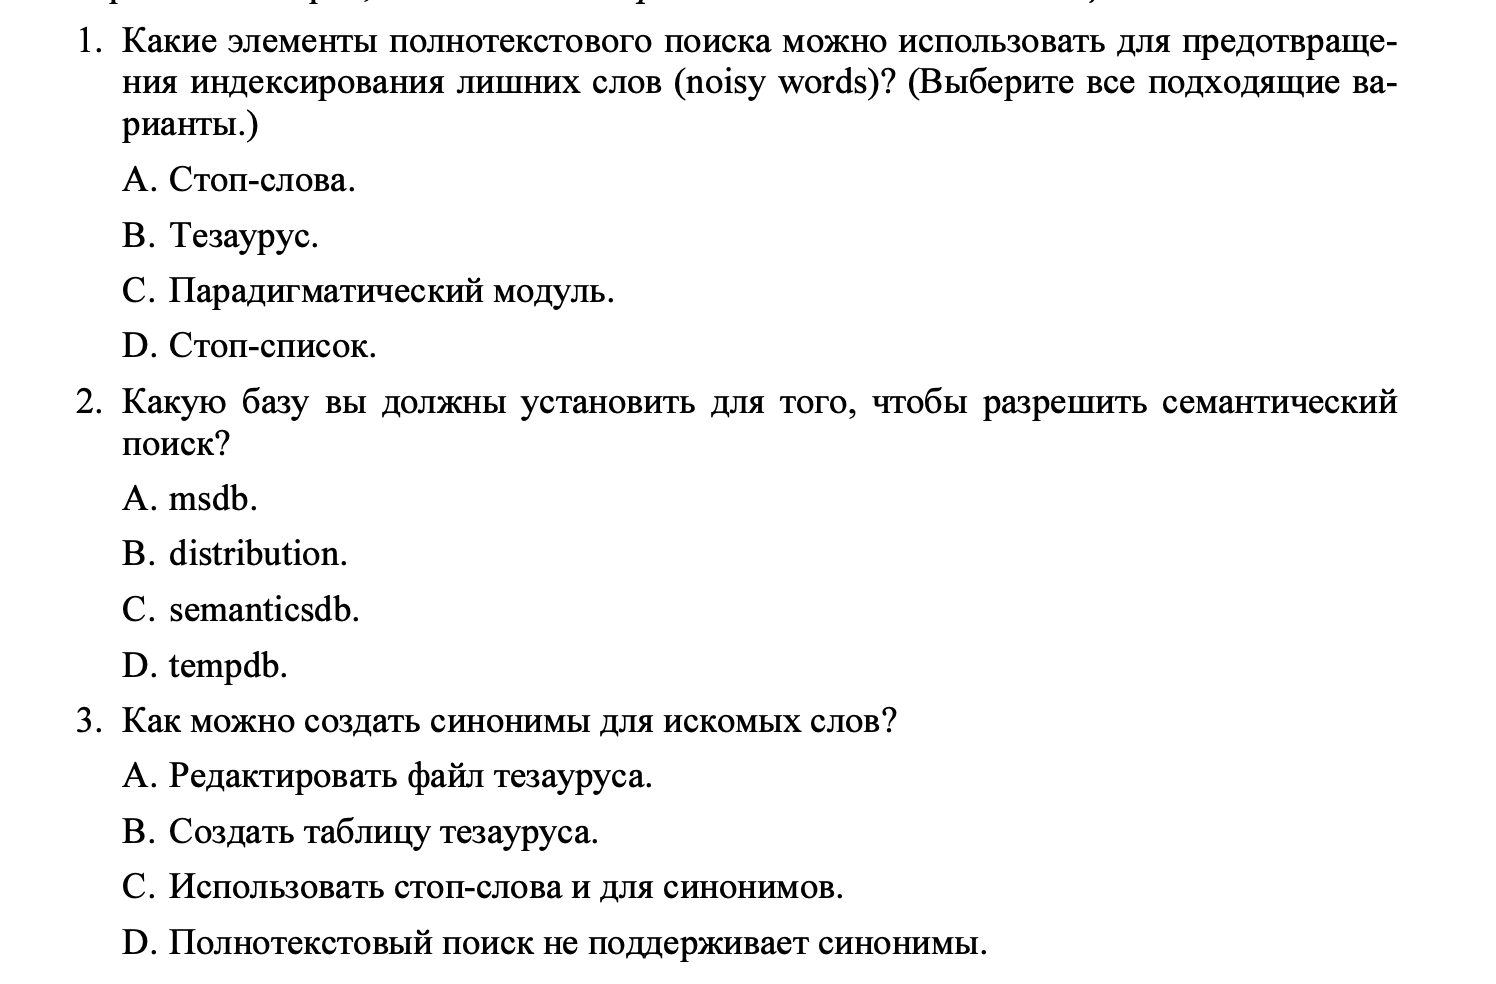
\includegraphics[width=0.8\textwidth]{img/zakrep14.png}
	\end{center}
	\captionsetup{justification=centering}
\end{figure}

\subsection*{Ответы}

\begin{figure}[h!]
	\begin{center}
		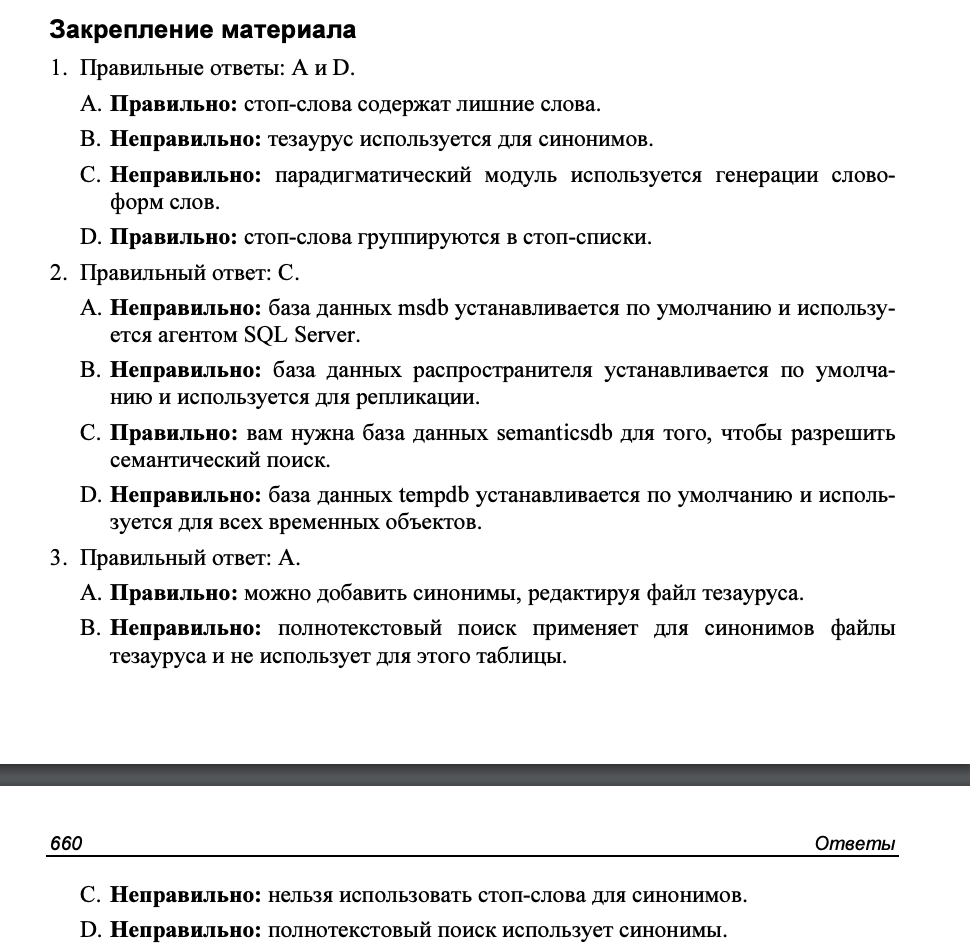
\includegraphics[width=0.9\textwidth]{img/ans15.png}
	\end{center}
	\captionsetup{justification=centering}
\end{figure}
\clearpage


\section{Использование предикатов CONTAINS и FREETEXT}

\subsection{Предикат CONTAINS}

Предикат CONTAINS предоставляет возможность выполнять поиск: 

\begin{itemize}
	\item слов и фраз в тексте;
	\item точных или примерных (fuzzy) совпадений; 
	\item словоформ слова; 
	\item текста, в котором искомое слово находится рядом с другим искомым словом; 
	\item синонимов искомого слова; 
	\item префикс слова или выражения. 
\end{itemize}


\subsection{Предикат FREETEXT}
Предикат FREETEXT является менее определенным и поэтому возвращает большее
число строк, чем предикат CONTAINS. Он выполняет поиск значений, совпадающих
со смыслом фразы, а не с точным значением слов. Когда вы используете предикат
FREETEXT, ядро выполняет разбиение на слова искомой фразы, генерирует словоформы (но не парадигмы) и определяет список расширений и замен для слов в выражениях поиска на основании слов из тезауруса. 


\subsection*{Резюме занятия}
\begin{itemize}
	\item Предикат CONTAINS можно использовать для избирательного поиска. 
	\item Предикат FREETEXT можно использовать для более общего поиска. 
\end{itemize}




\section{Использование табличных функций полнотекстового и семантического поиска}

\subsection{Статистические оконные функции}
\begin{itemize}
	\item SEMANTICKEYPHRASETABLE
	\item SEMANTICSIMILARITYDETAILSTABLE
	\item SEMANTICSIMILARITYTABLE
\end{itemize}

